\chapter{Algoritmos completos}

\section{Obtención de celdas base}\label{algComp:celdasbase}
El algoritmo \ref{alg:celdasBaseCompleto} es una versión del algoritmo \ref{alg:celdasBase} sin las
simplificaciones comentadas en la sección \ref{subsec:critPer}.

\begin{algorithm}[H]
\SetAlgoLined
  \SetKwInOut{Input}{Entrada}
  \Input{$c$}

% En updateBase c es pN y cA es p
% En setPseudoSourcesFromWave c es p y cA es waveP
  % \tcp{DFS desde $c$ agregando las celdas visitadas a la componente conexa $C_i$}
  $\mli{CB}_c := \emptyset$

  \ForEach{ $cA \in ady(c)$} {
    \ForEach{$b \in gens(cA)$} {
      $\mli{tolerado}  := d_c(b) \leq \mli{DD}(c) + L$\\
      % $\mli{noIgNiAdy} := b \notin gens(c) \land b \notin \bigcup_{b'} ady(gen(c))$\\

      $\mli{masCercano} := verdadero$\\
      $\mli{aRemover} := \emptyset$\\
      % \ForEach{$b' \in \mli{CB}_c$ \textbf{mientras} masCercano } {
      \ForEach{$b' \in \mli{CB}_c$} {
        \If{$b' = b \lor b' \in ady(b)$}{
          \uIf{$d_c(b) < d_c(b')$}{
            $\mli{aRemover} := \mli{aRemover} \cup \{b'\}$\\
          }\Else{
            $\mli{masCercano} := \mli{masCercano} \land falso$ \\
            \tcp{No es necesario continuar con la iteración de la línea 7 una vez ejecutada esta línea}
          }
        }
      }
      
      \If{tolerado $\land$ masCercano}{
        $\mli{CB}_c := \mli{CB}_c -\mli{aRemover}$\\
        $\mli{CB}_c := \mli{CB}_c \cup \{\mli{b}\}$\\
      }
    }
  }
  \Return $\mli{CB}_c$ 

  \caption{Obtención de las celdas base $\mli{CB}_c$ de una celda $c$}
  \label{alg:celdasBaseCompleto}
\end{algorithm}

\newpage
Uno de los principales cambios respecto al algoritmo \ref{alg:celdasBase} es el
remplazo de la función $gen$ por la función $gens : \mli{CG} \rightarrow
P(\mli{CGen})$ que dada una celda $c$ de la grilla devuelve el conjunto de
todas las celdas que pertenecen a un generador que están a mínima distancia de
$c$. Otro cambio a notar es que la condición asociada a la variable
$\mli{masCercano}$ (líneas 5-15) pasa a ser que la celda base candidata $b$
esté a menor distancia de $c$ que las celdas base actuales $b'$ que son
iguales o adyacentes a $b$. El último cambio a destacar es que la condición que
en algoritmo \ref{alg:celdasBase} se controla con la variable
$\mli{noIgNiAdy}$, en este algoritmo se controla a partir las variables
$\mli{masCercano}$ y $\mli{aRemover}$.
% en la condición
% asociada a la variable $\mli{masCercano}$
% y de cumplirse todas las
% condiciones los $b'$ adyacentes a $b$ dejan de ser celdas base de $c$.
\newpage

\chapter{Ejemplos completos}
\begingroup
\small
\section{Obtención de fronteras significativas basada en cubrimiento}\label{EXE:sfbc}
La figura \ref{EXE:sfbc} presenta la versión completa del ejemplo mostrado en la figura \ref{fig:ejemploFSCub}.
\endgroup
\begin{figure}[H]
  \centerfloat
  \subfloat[Estado inicial.]{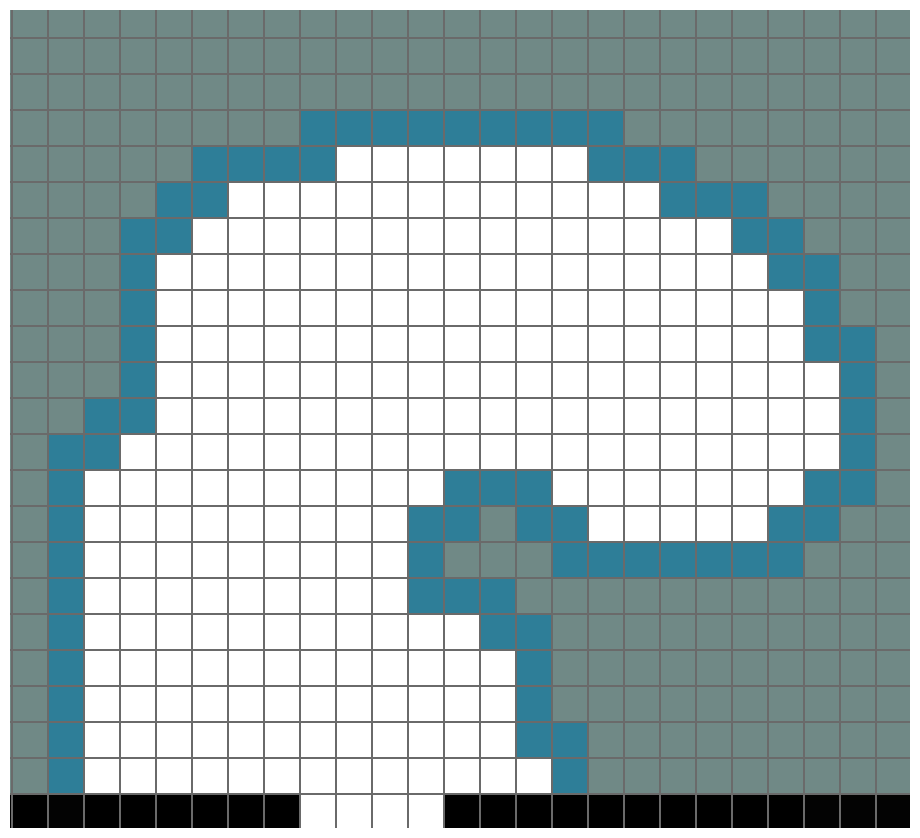
\includegraphics[clip=true, width=0.48\textwidth]{imagenes/ejemploSimpCub/a1.png}}
  \subfloat[Se inicializa $\mli{FP}$.]{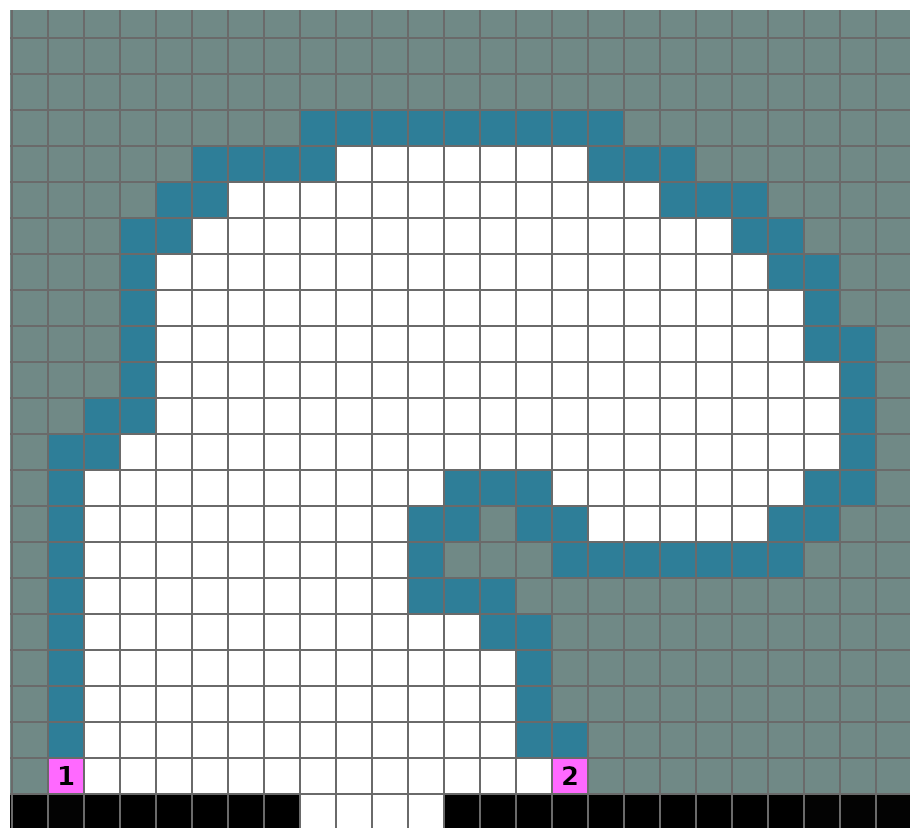
\includegraphics[clip=true, width=0.48\textwidth]{imagenes/ejemploSimpCub/a2.png}}

  \subfloat[Se obtiene $\mli{fp}$ desencolando de $\mli{FP}$.]{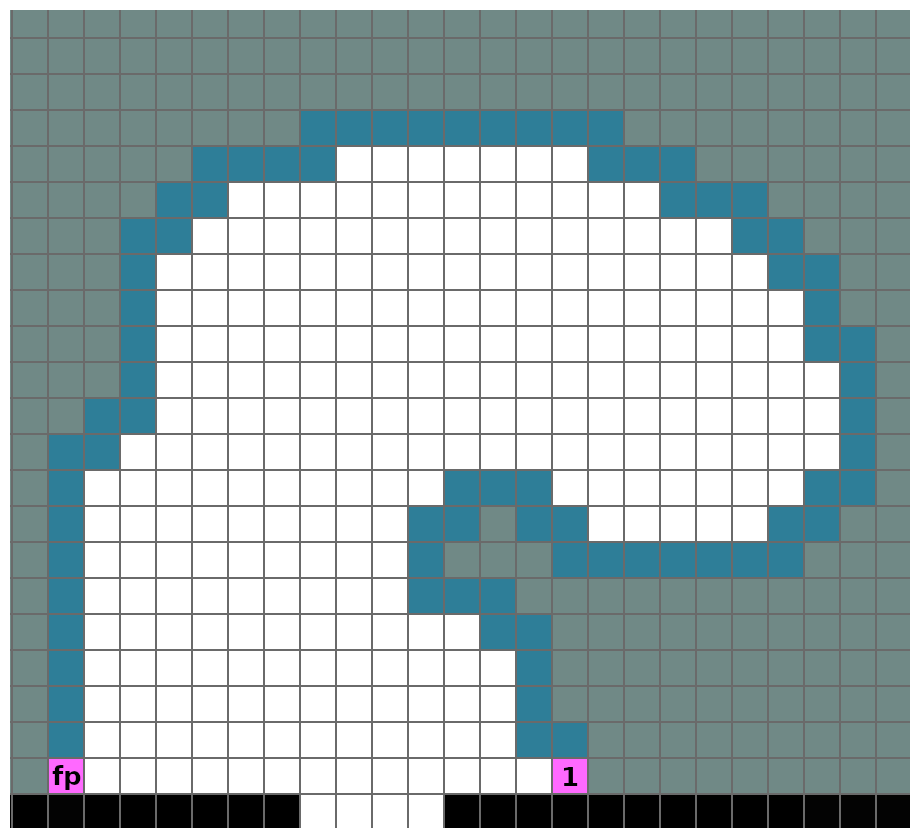
\includegraphics[clip=true, width=0.40\textwidth]{imagenes/ejemploSimpCub/b1.png}}
  \subfloat[Existen celdas en $\mli{UF}$ a una distancia mayor que $2*rango$ de $\mli{fp}$, los candidatos se obtienen con $radio=rango$. ]{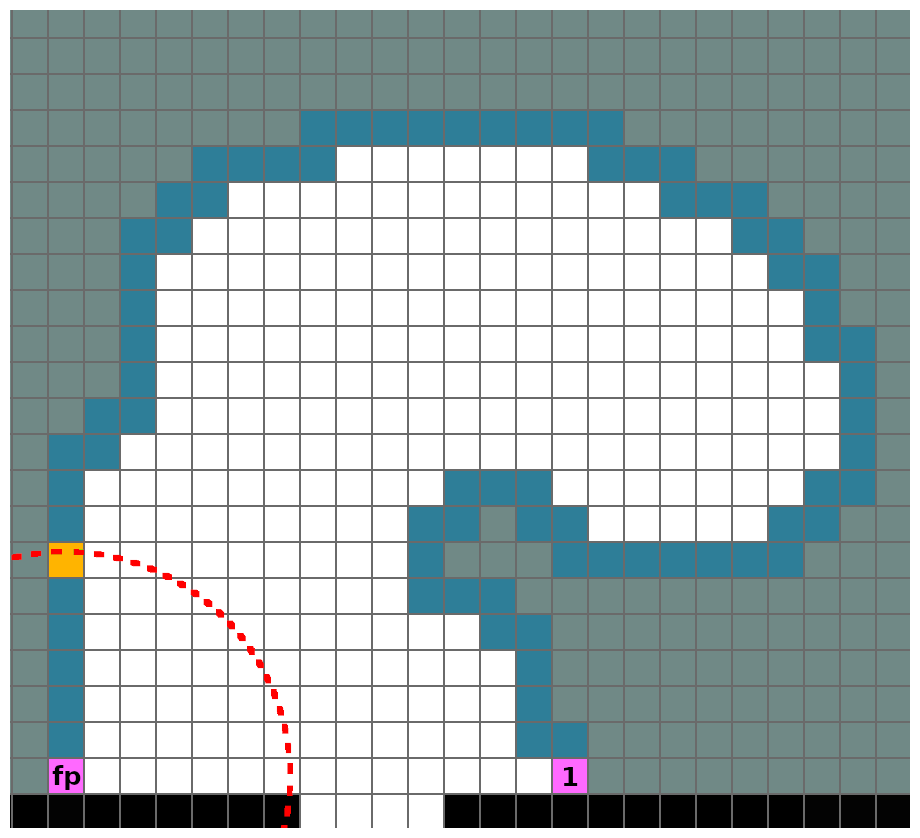
\includegraphics[clip=true, width=0.40\textwidth]{imagenes/ejemploSimpCub/b3.png}}
  \subfloat[Se elige el único candidato como $\mli{fs}$, se actualiza $\mli{UF}$, $\mli{FS_i}$ y $\mli{FP}$.]{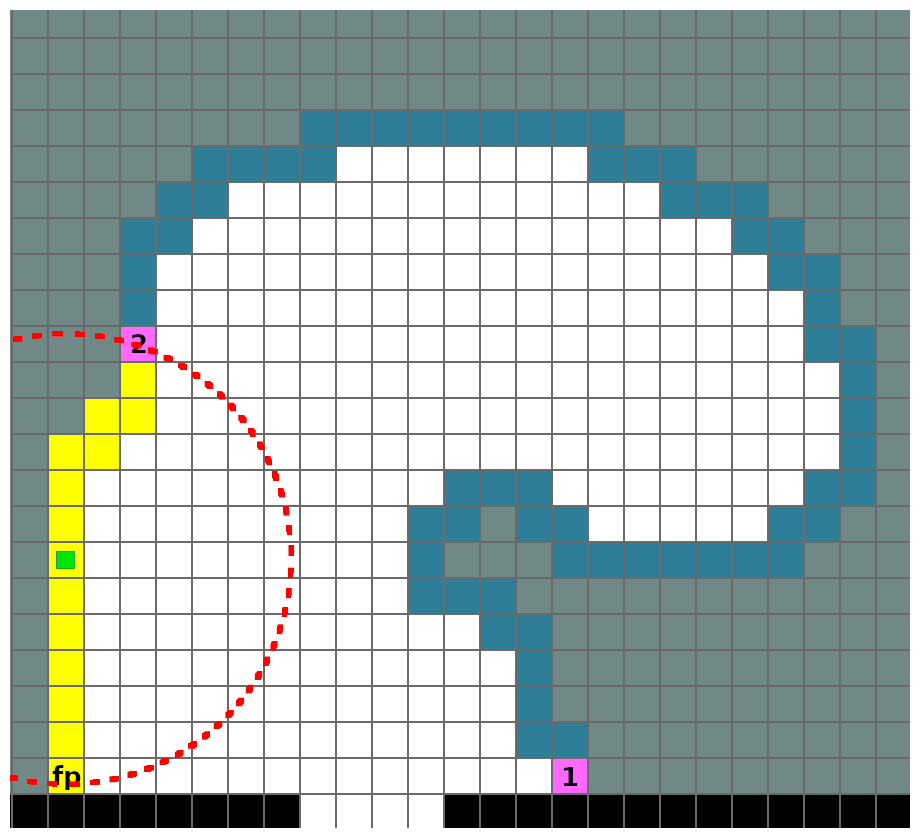
\includegraphics[clip=true, width=0.40\textwidth]{imagenes/ejemploSimpCub/b5.png}}

 \phantomcaption

\end{figure}

\begin{figure}[H]
  \setcounter{subfigure}{5}
  \centerfloat

  \subfloat[Se obtiene $\mli{fp}$ desencolando de $\mli{FP}$.]{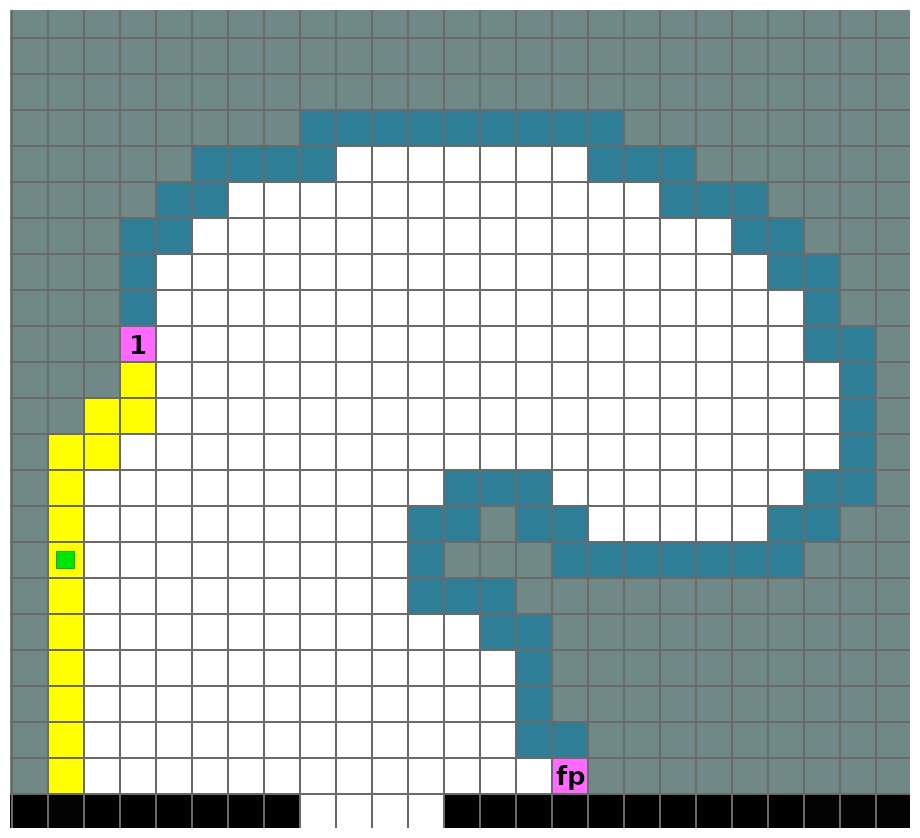
\includegraphics[clip=true, width=0.40\textwidth]{imagenes/ejemploSimpCub/c1.png}}
  \subfloat[Existen celdas en $\mli{UF}$ a una distancia mayor que $2*rango$ de $\mli{fp}$, los candidatos se obtienen con $radio=rango$. ]{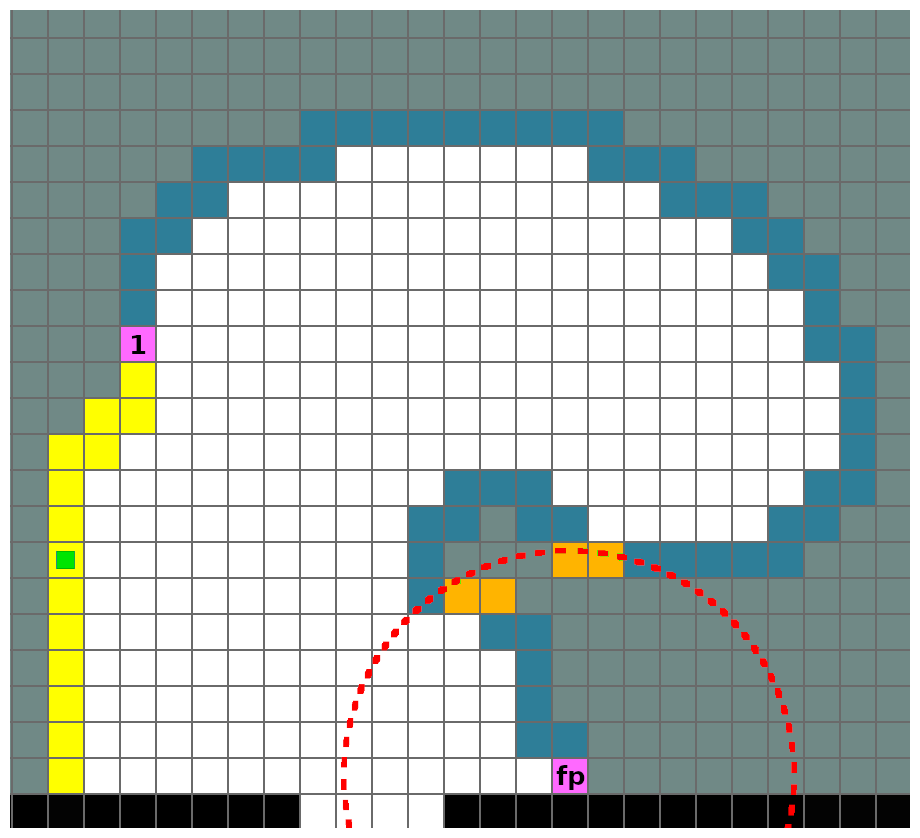
\includegraphics[clip=true, width=0.40\textwidth]{imagenes/ejemploSimpCub/c3.png}}
  \subfloat[Se elige arbitrariamente un candidato como $\mli{fs}$, se actualiza $\mli{UF}$, $\mli{FS_i}$ y $\mli{FP}$.]{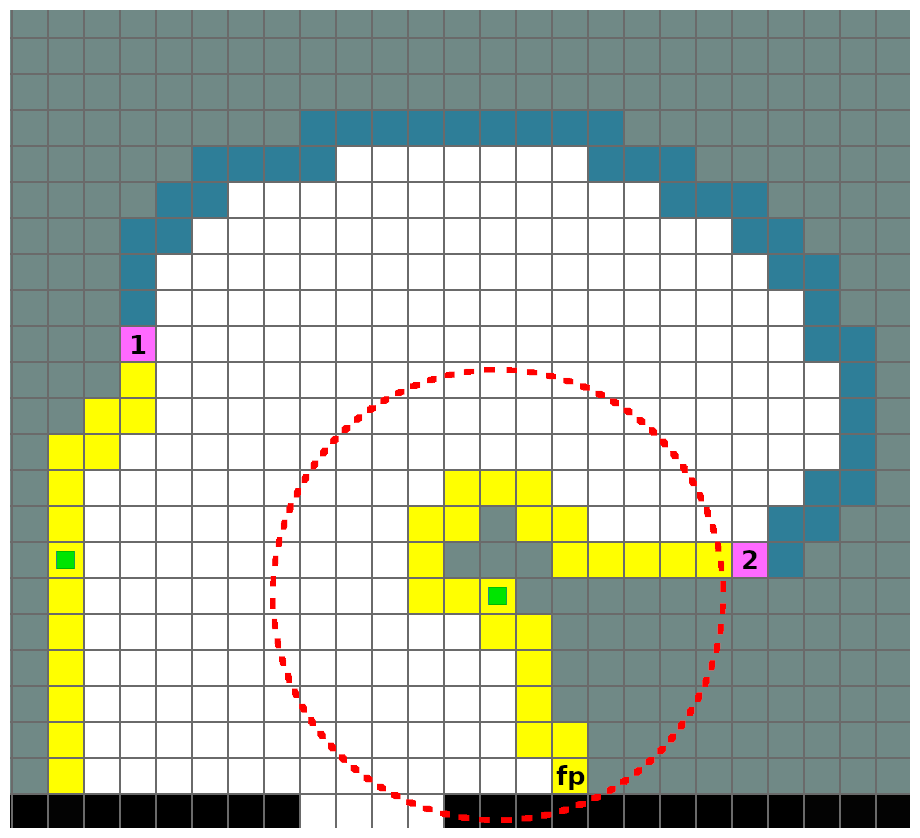
\includegraphics[clip=true, width=0.40\textwidth]{imagenes/ejemploSimpCub/c5.png}}


  \subfloat[Se obtiene $\mli{fp}$ desencolando de $\mli{FP}$.]{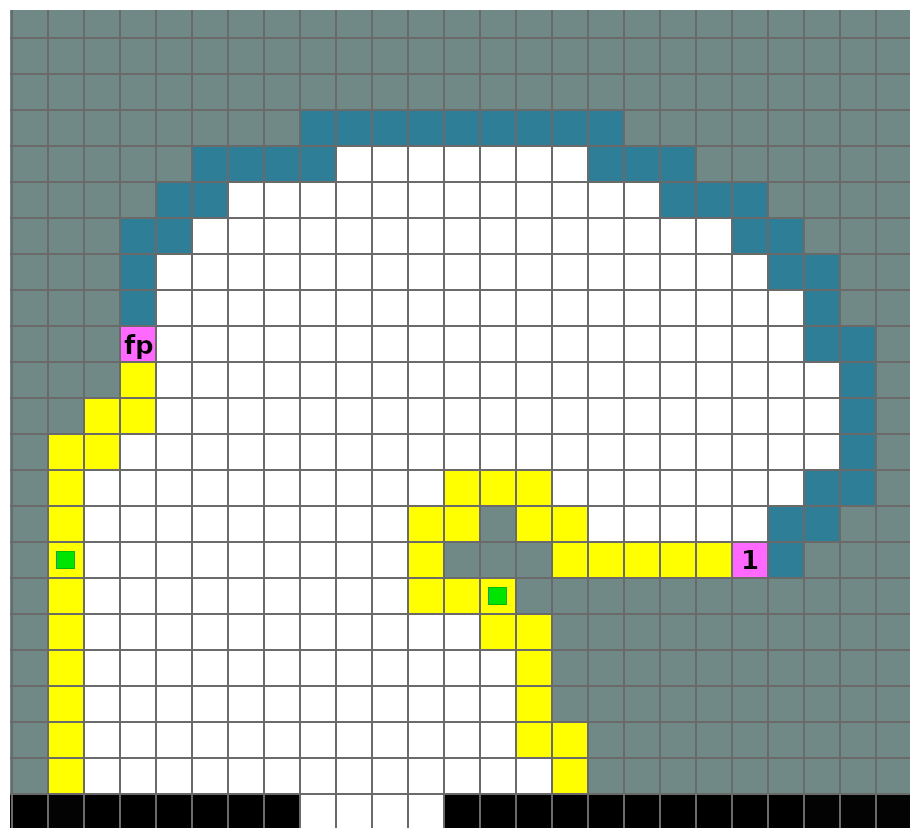
\includegraphics[clip=true, width=0.40\textwidth]{imagenes/ejemploSimpCub/d1.png}}
  \subfloat[Existen celdas en $\mli{UF}$ a una distancia mayor que $2*rango$ de $\mli{fp}$, los candidatos se obtienen con $radio=rango$. ]{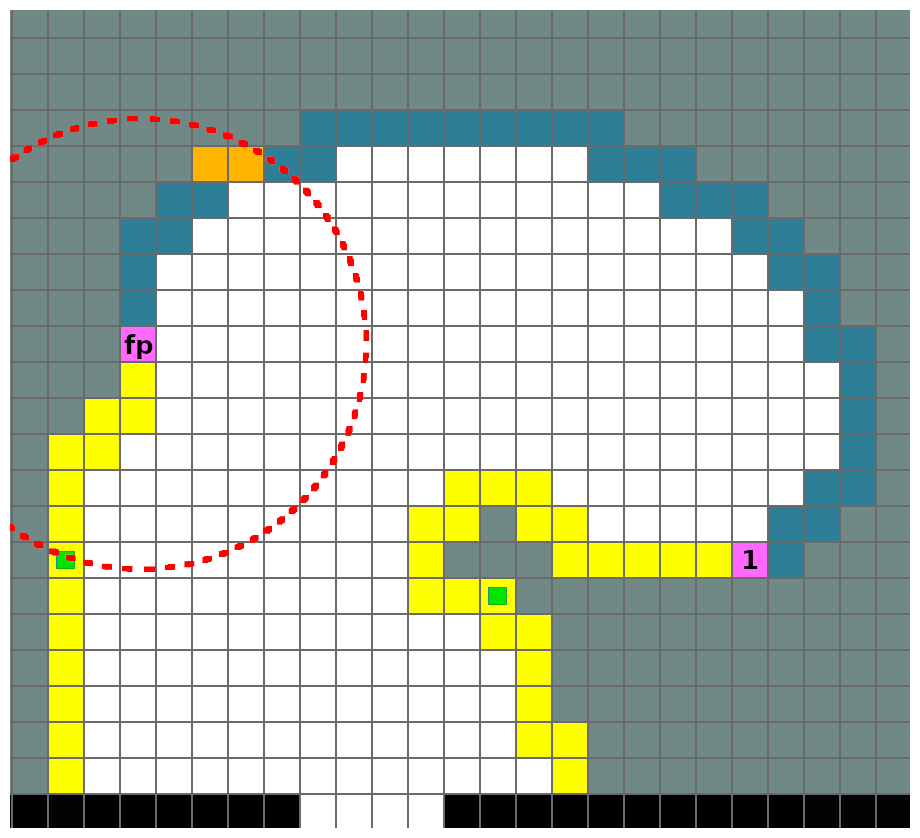
\includegraphics[clip=true, width=0.40\textwidth]{imagenes/ejemploSimpCub/d3.png}}
  \subfloat[Se elige arbitrariamente un candidato como $\mli{fs}$, se actualiza $\mli{UF}$, $\mli{FS_i}$ y $\mli{FP}$.]{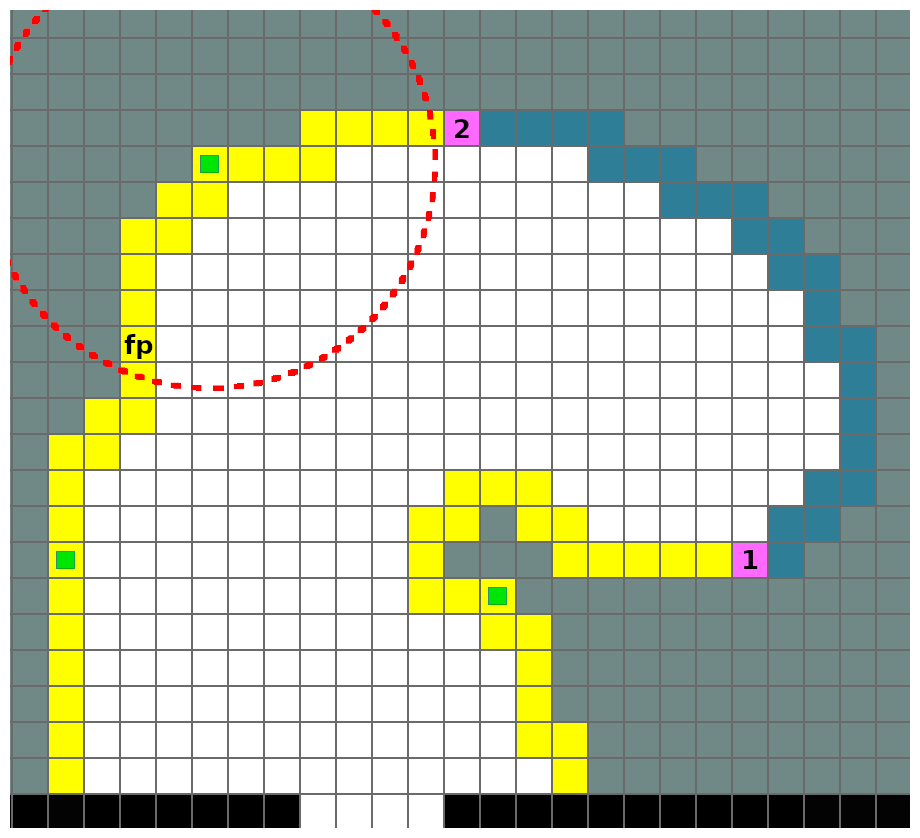
\includegraphics[clip=true, width=0.40\textwidth]{imagenes/ejemploSimpCub/d5.png}}

  \subfloat[Se obtiene $\mli{fp}$ desencolando de $\mli{FP}$.]{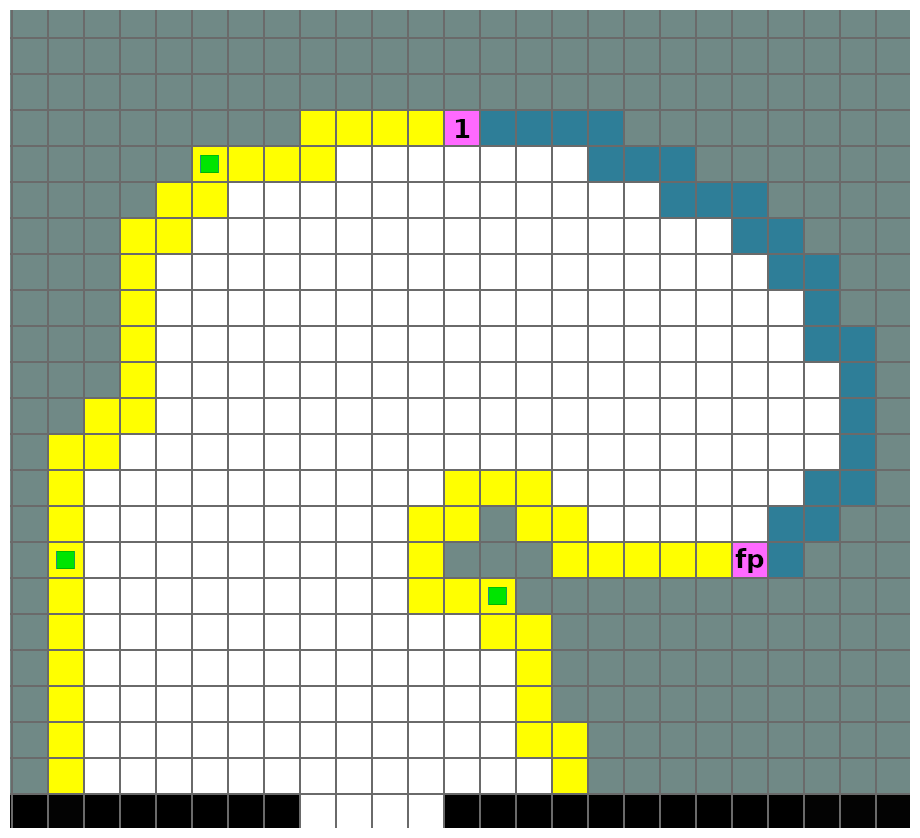
\includegraphics[clip=true, width=0.40\textwidth]{imagenes/ejemploSimpCub/e1.png}}
  \subfloat[Existen celdas en $\mli{UF}$ a una distancia mayor que $2*rango$ de $\mli{fp}$, los candidatos se obtienen con $radio=rango$. ]{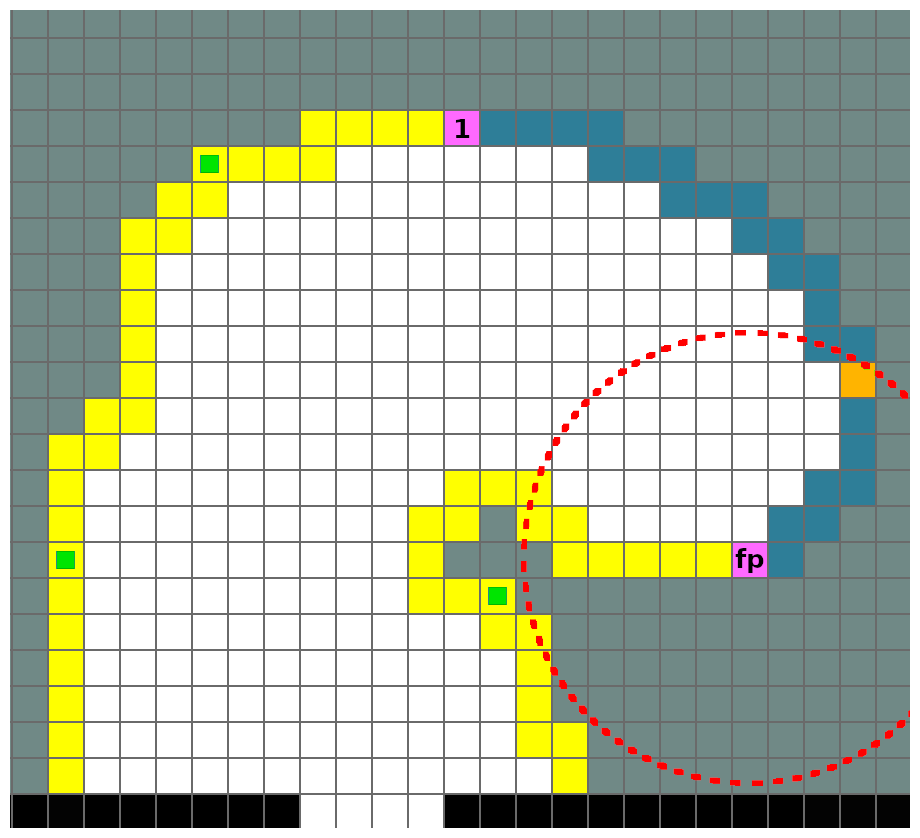
\includegraphics[clip=true, width=0.40\textwidth]{imagenes/ejemploSimpCub/e3.png}}
  \subfloat[Se elige el único candidato como $\mli{fs}$, se actualiza $\mli{UF}$, $\mli{FS_i}$ y $\mli{FP}$.]{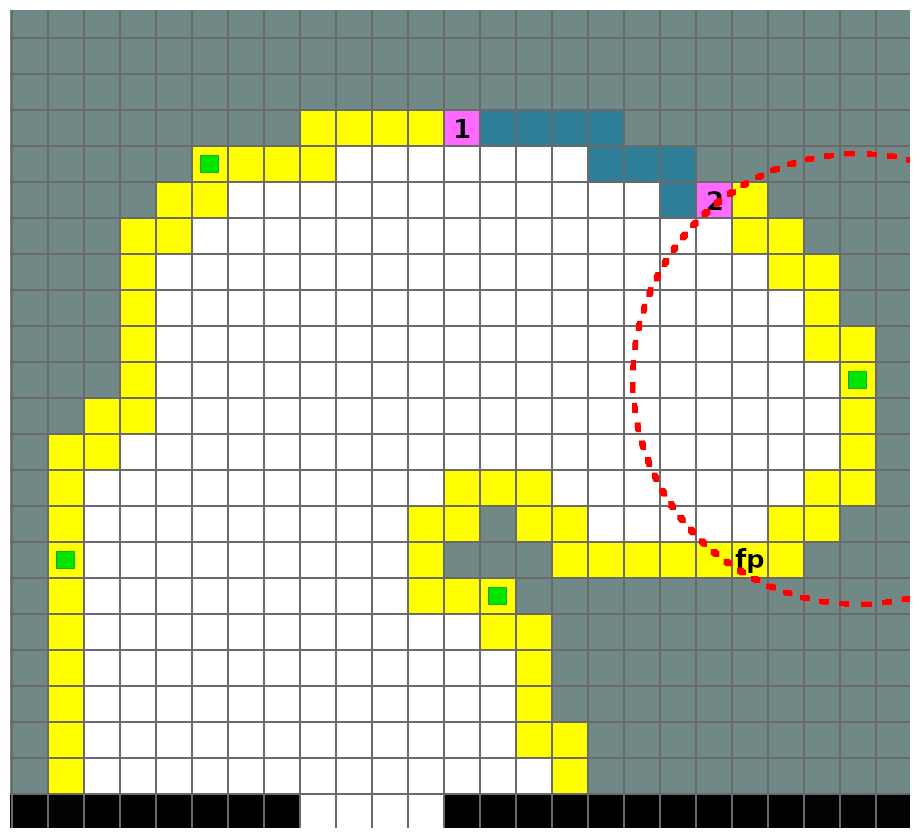
\includegraphics[clip=true, width=0.40\textwidth]{imagenes/ejemploSimpCub/e5.png}}


 \phantomcaption
\end{figure}

\setcounter{figure}{0}

\begin{figure}[H]
  \setcounter{subfigure}{14}
  \centerfloat

  \subfloat[Se obtiene $\mli{fp}$ desencolando de $\mli{FP}$.]{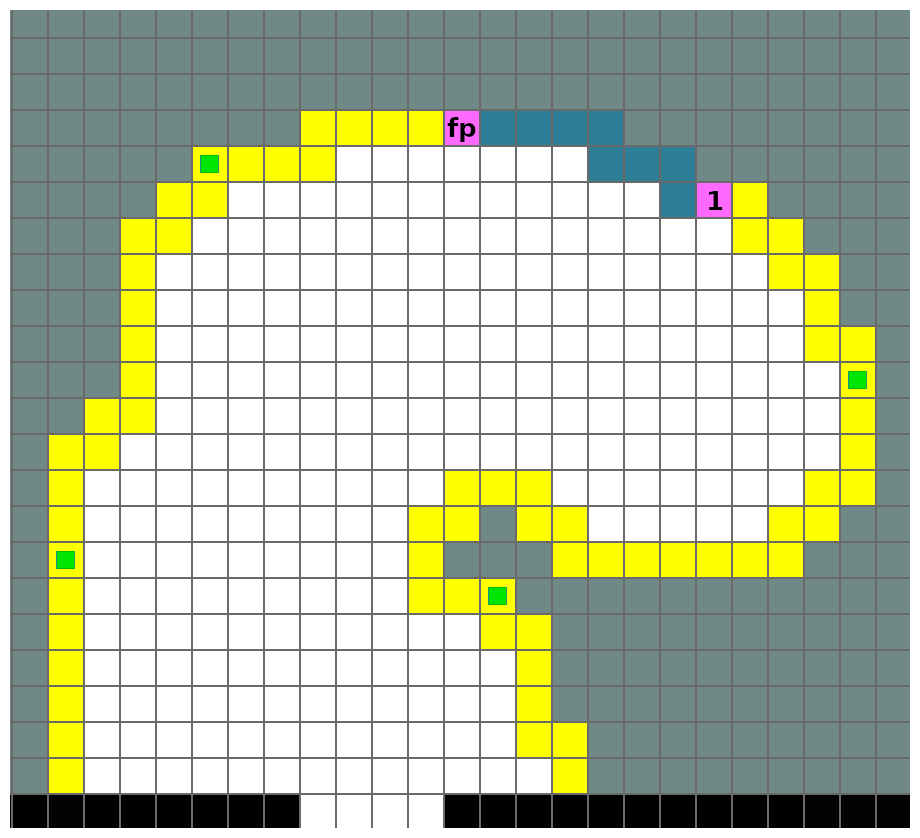
\includegraphics[clip=true, width=0.40\textwidth]{imagenes/ejemploSimpCub/f1.png}}
  \subfloat[No existen celdas en $\mli{UF}$ a una distancia mayor que $2*rango$ de $\mli{fp}$, la celda de $\mli{UF}$ más alejada está a $\smallsim7.4$ (largos de celda), los candidatos se obtienen con $radio\cong3.7$ (largos de celda). ]{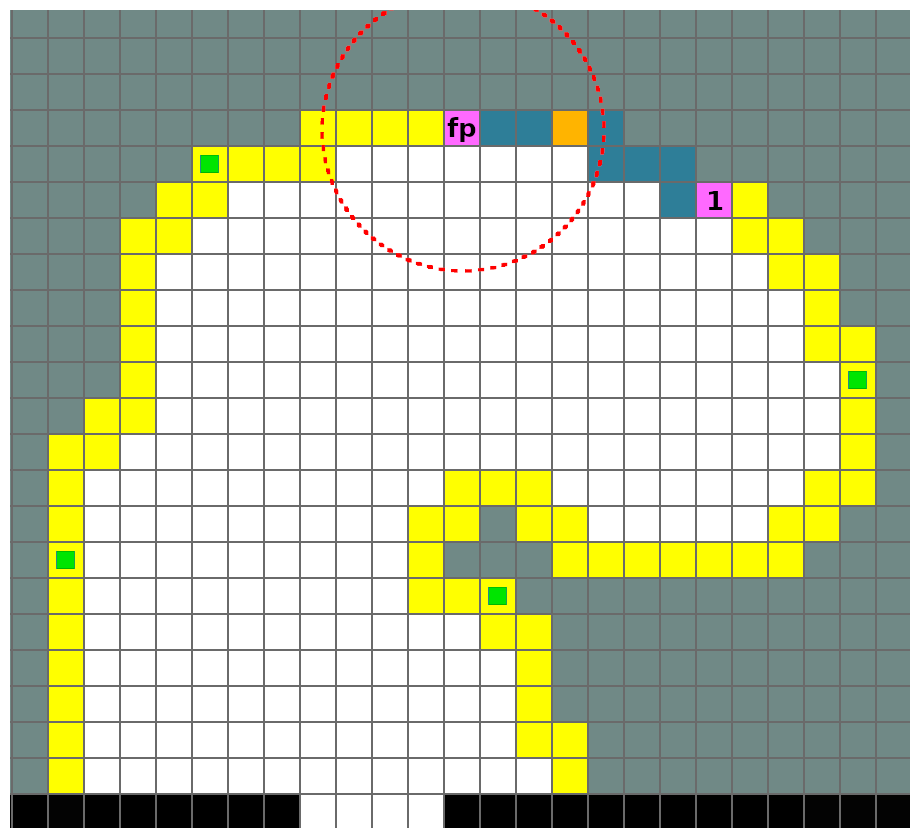
\includegraphics[clip=true, width=0.40\textwidth]{imagenes/ejemploSimpCub/f3.png}}
  \subfloat[Se elige el único candidato como $\mli{fs}$, se actualiza $\mli{UF}$, $\mli{FS_i}$ y $\mli{FP}$.]{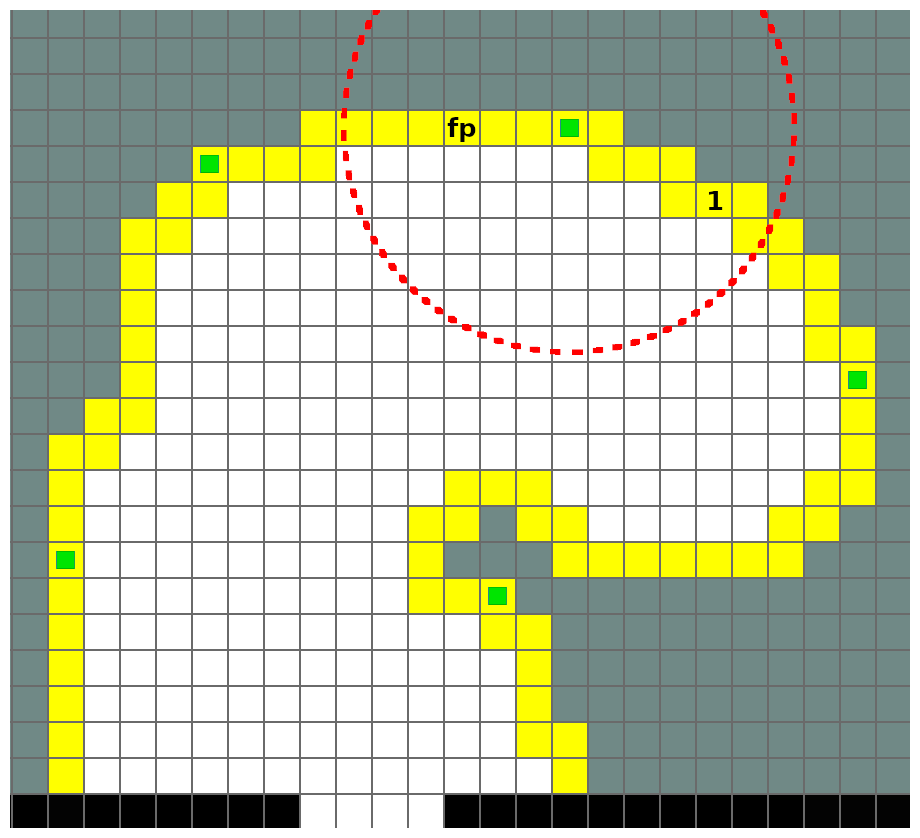
\includegraphics[clip=true, width=0.40\textwidth]{imagenes/ejemploSimpCub/f4.png}}


  \subfloat[$\mli{UF}=\emptyset$ por lo que el algoritmo finaliza.]{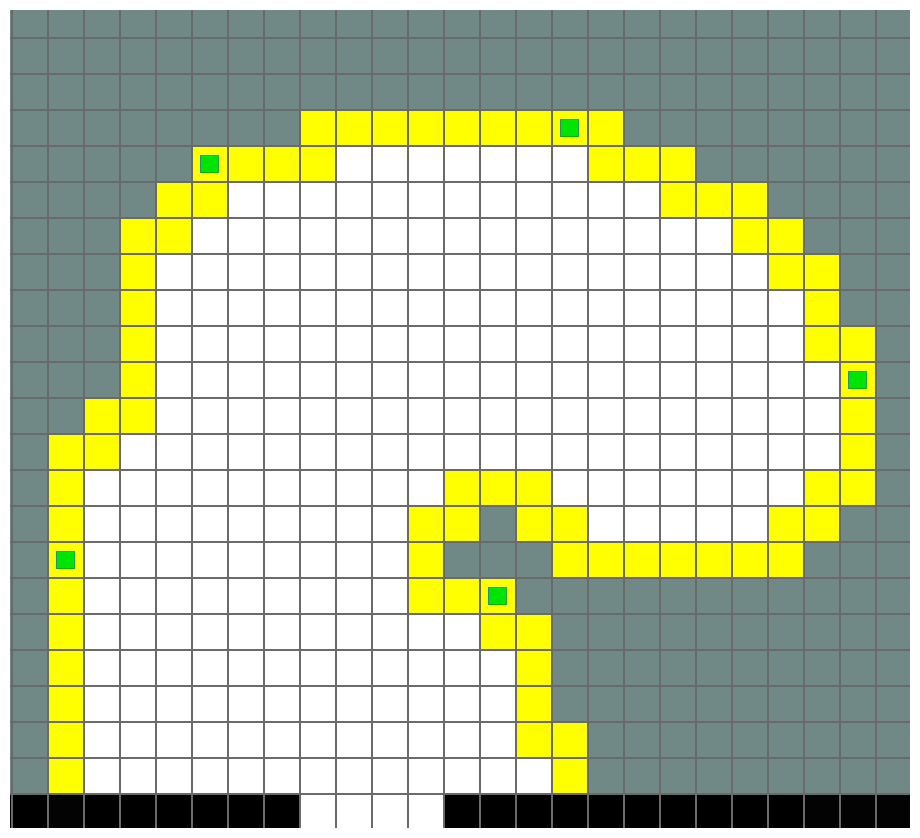
\includegraphics[clip=true, width=0.40\textwidth]{imagenes/ejemploSimpCub/zfinal1.png}}
  \subfloat[Se logra el cubrimiento.]{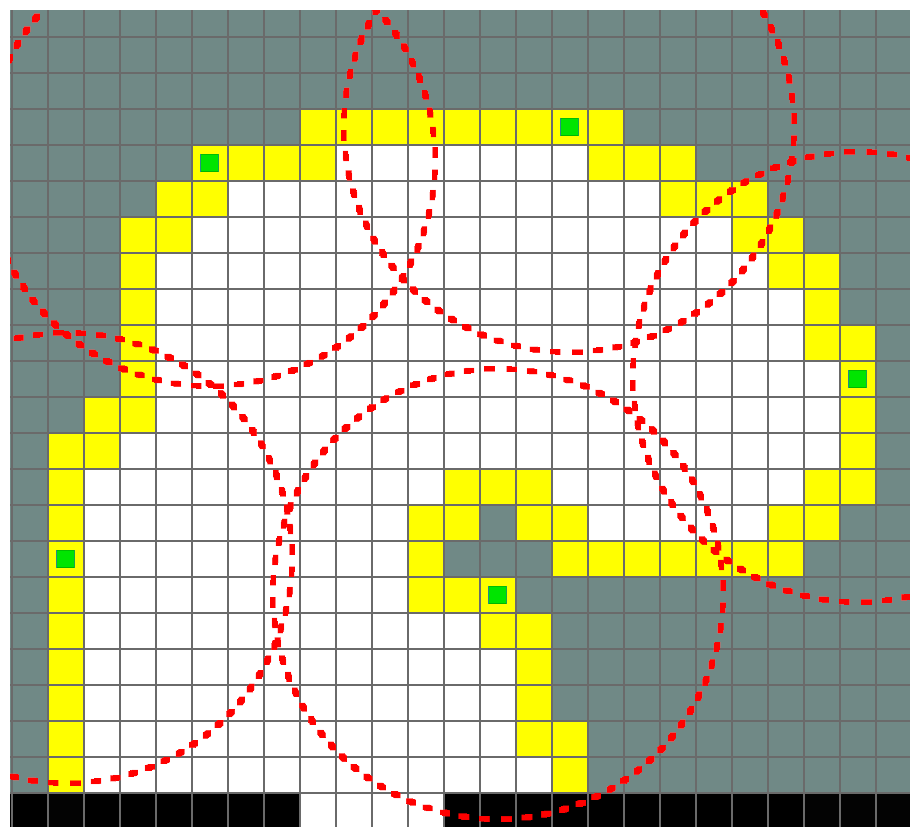
\includegraphics[clip=true, width=0.40\textwidth]{imagenes/ejemploSimpCub/zfinal2.png}}
  % \subfloat[$\mli{UF}=\emptyset$ por lo que el algoritmo finaliza.]{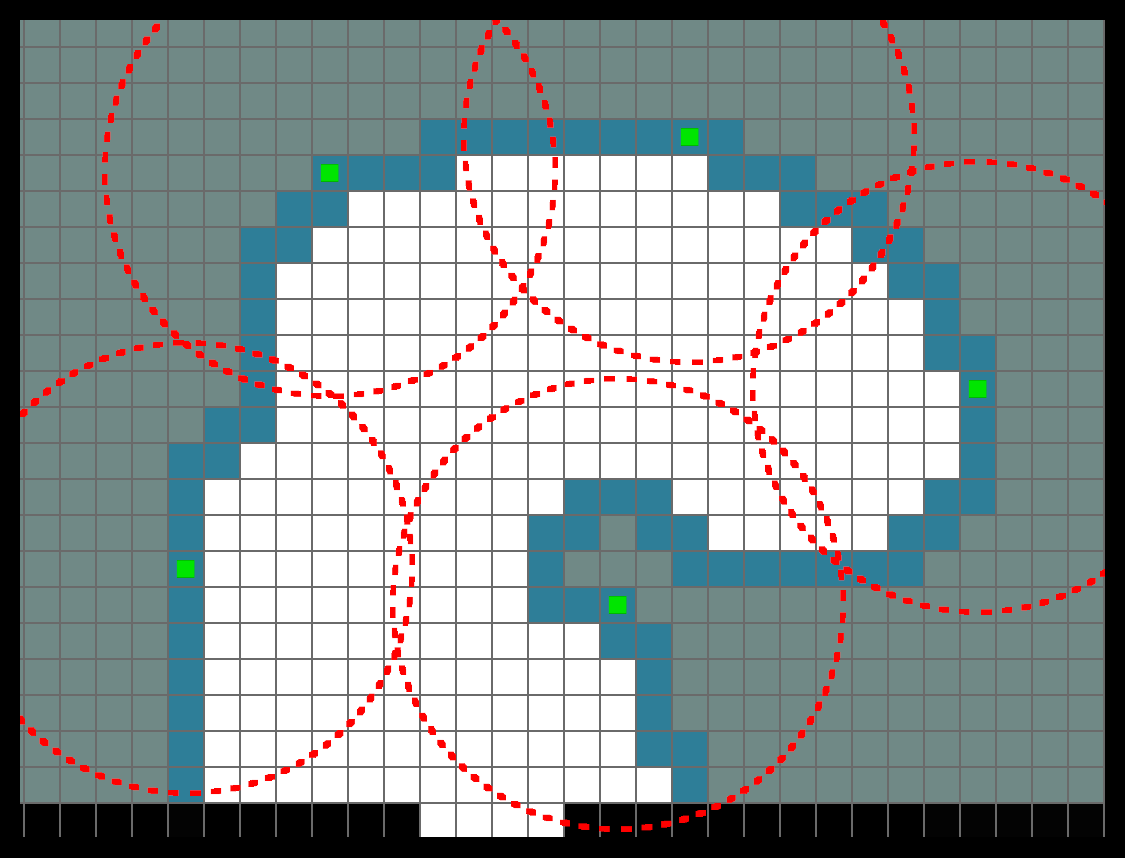
\includegraphics[clip=true, width=0.40\textwidth]{imagenes/ejemploSimpCub/zfinal3.png}}

  \caption[Proceso de obtención de fronteras significativas basado en cubrimiento.]{Proceso
    de obtención de fronteras significativas basado en cubrimiento. Las fronteras de $F_i$ se
    indican con azul si pertenecen a $\mli{UF}$ y con amarillo de lo contrario.
    Con magenta se indican las celdas en $\mli{FP}$ siendo la numeración su
    orden en la cola y $\mli{fp}$ la última desencolada. Las
    circunferencias rojas centradas en $\mli{fp}$ tienen como radio la distancia
    utilizada para obtener los candidatos $\mli{FSC}$ los cuales se indican con
    naranja. Las fronteras significativas se indican con verde, siendo las
    circunferencias rojas de radio $rango=5.6$ (largos de celda) centradas en estas indicadores de su
  cubrimiento.}\label{fig:ejemploFSCubComp}

\end{figure}
